% Created by tikzDevice version 0.12.6 on 2024-04-14 21:43:58
% !TEX encoding = UTF-8 Unicode
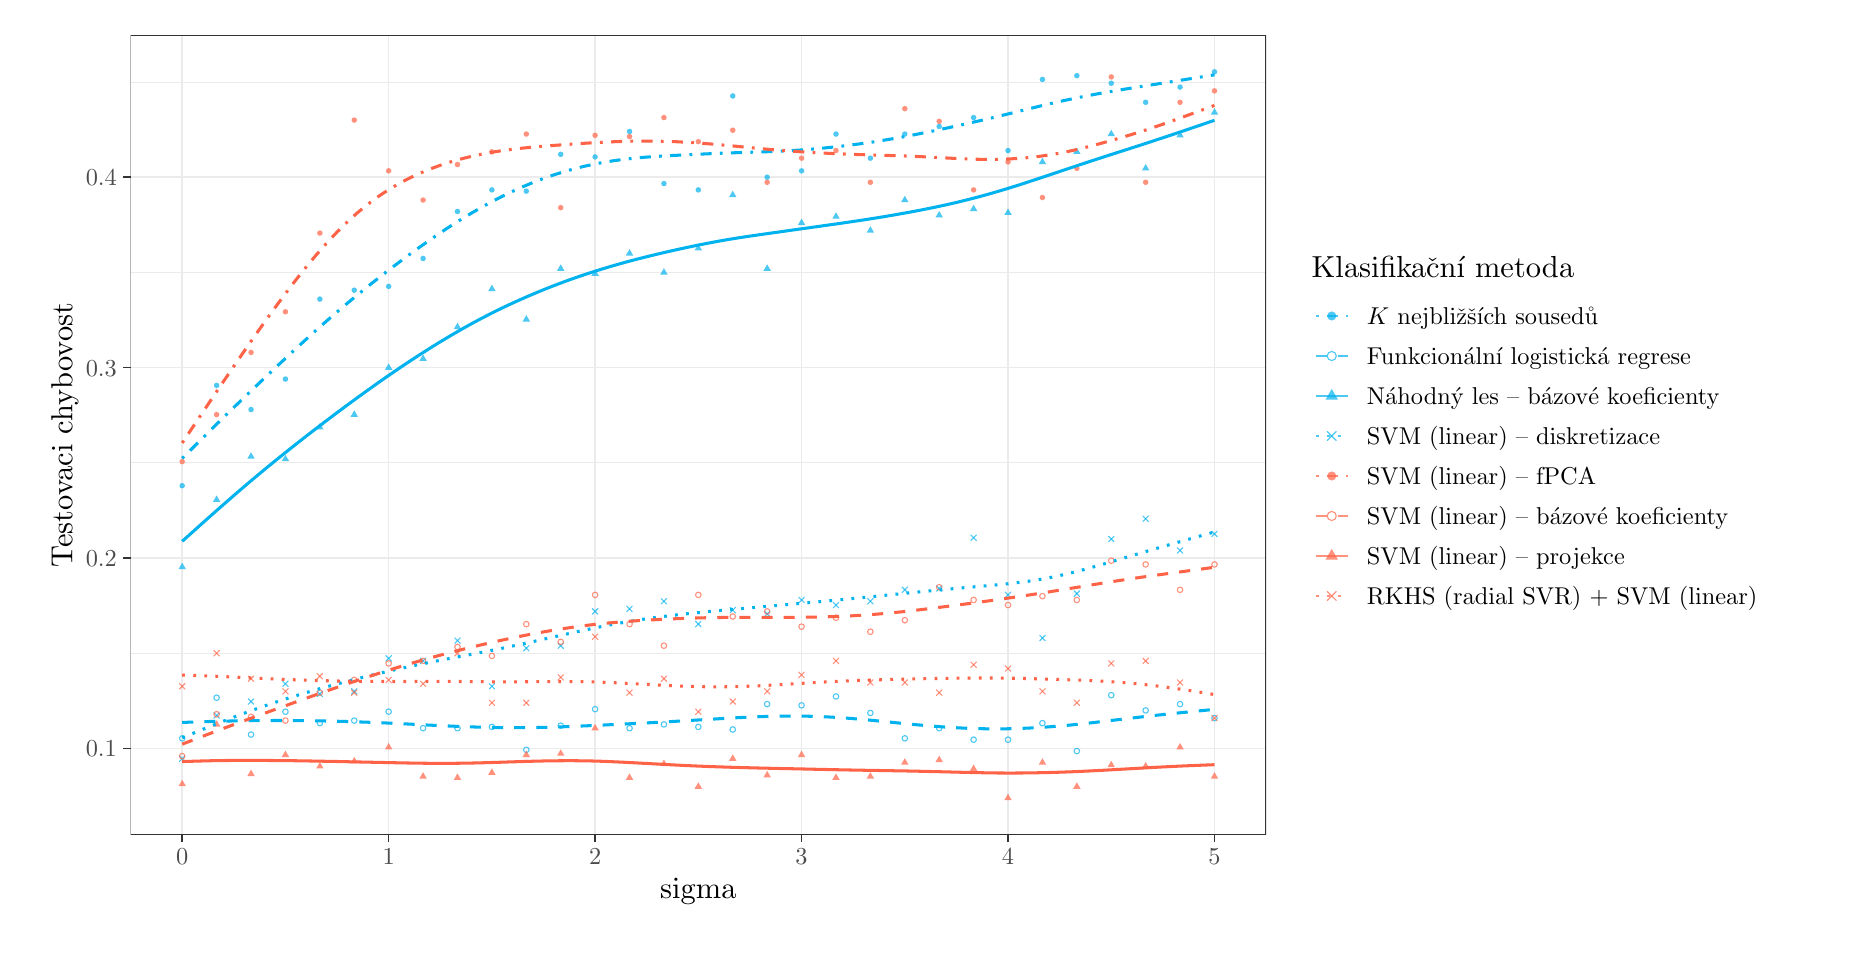
\begin{tikzpicture}[x=1pt,y=1pt]
\definecolor{fillColor}{RGB}{255,255,255}
\path[use as bounding box,fill=fillColor] (0,0) rectangle (650.43,325.21);
\begin{scope}
\path[clip] (  0.00,  0.00) rectangle (650.43,325.21);
\definecolor{drawColor}{RGB}{255,255,255}

\path[draw=drawColor,line width= 0.6pt,line join=round,line cap=round,fill=fillColor] (  0.00,  0.00) rectangle (650.43,325.21);
\end{scope}
\begin{scope}
\path[clip] ( 37.19, 33.72) rectangle (447.50,322.37);
\definecolor{fillColor}{RGB}{255,255,255}

\path[fill=fillColor] ( 37.19, 33.72) rectangle (447.50,322.37);
\definecolor{drawColor}{gray}{0.92}

\path[draw=drawColor,line width= 0.3pt,line join=round] ( 37.19, 99.14) --
	(447.50, 99.14);

\path[draw=drawColor,line width= 0.3pt,line join=round] ( 37.19,167.95) --
	(447.50,167.95);

\path[draw=drawColor,line width= 0.3pt,line join=round] ( 37.19,236.77) --
	(447.50,236.77);

\path[draw=drawColor,line width= 0.3pt,line join=round] ( 37.19,305.58) --
	(447.50,305.58);

\path[draw=drawColor,line width= 0.6pt,line join=round] ( 37.19, 64.73) --
	(447.50, 64.73);

\path[draw=drawColor,line width= 0.6pt,line join=round] ( 37.19,133.55) --
	(447.50,133.55);

\path[draw=drawColor,line width= 0.6pt,line join=round] ( 37.19,202.36) --
	(447.50,202.36);

\path[draw=drawColor,line width= 0.6pt,line join=round] ( 37.19,271.17) --
	(447.50,271.17);

\path[draw=drawColor,line width= 0.6pt,line join=round] ( 55.84, 33.72) --
	( 55.84,322.37);

\path[draw=drawColor,line width= 0.6pt,line join=round] (130.44, 33.72) --
	(130.44,322.37);

\path[draw=drawColor,line width= 0.6pt,line join=round] (205.04, 33.72) --
	(205.04,322.37);

\path[draw=drawColor,line width= 0.6pt,line join=round] (279.65, 33.72) --
	(279.65,322.37);

\path[draw=drawColor,line width= 0.6pt,line join=round] (354.25, 33.72) --
	(354.25,322.37);

\path[draw=drawColor,line width= 0.6pt,line join=round] (428.85, 33.72) --
	(428.85,322.37);
\definecolor{fillColor}{RGB}{0,178,238}

\path[fill=fillColor,fill opacity=0.70] ( 55.84,159.70) circle (  1.00);

\path[fill=fillColor,fill opacity=0.70] ( 68.28,195.94) circle (  1.00);

\path[fill=fillColor,fill opacity=0.70] ( 80.71,187.22) circle (  1.00);

\path[fill=fillColor,fill opacity=0.70] ( 93.14,198.23) circle (  1.00);

\path[fill=fillColor,fill opacity=0.70] (105.58,227.13) circle (  1.00);

\path[fill=fillColor,fill opacity=0.70] (118.01,230.34) circle (  1.00);

\path[fill=fillColor,fill opacity=0.70] (130.44,231.72) circle (  1.00);

\path[fill=fillColor,fill opacity=0.70] (142.88,241.81) circle (  1.00);

\path[fill=fillColor,fill opacity=0.70] (155.31,258.79) circle (  1.00);

\path[fill=fillColor,fill opacity=0.70] (167.74,266.59) circle (  1.00);

\path[fill=fillColor,fill opacity=0.70] (180.18,266.13) circle (  1.00);

\path[fill=fillColor,fill opacity=0.70] (192.61,279.43) circle (  1.00);

\path[fill=fillColor,fill opacity=0.70] (205.04,278.51) circle (  1.00);

\path[fill=fillColor,fill opacity=0.70] (217.48,287.69) circle (  1.00);

\path[fill=fillColor,fill opacity=0.70] (229.91,268.88) circle (  1.00);

\path[fill=fillColor,fill opacity=0.70] (242.34,266.59) circle (  1.00);

\path[fill=fillColor,fill opacity=0.70] (254.78,300.53) circle (  1.00);

\path[fill=fillColor,fill opacity=0.70] (267.21,271.17) circle (  1.00);

\path[fill=fillColor,fill opacity=0.70] (279.65,273.47) circle (  1.00);

\path[fill=fillColor,fill opacity=0.70] (292.08,286.77) circle (  1.00);

\path[fill=fillColor,fill opacity=0.70] (304.51,278.05) circle (  1.00);

\path[fill=fillColor,fill opacity=0.70] (316.95,286.77) circle (  1.00);

\path[fill=fillColor,fill opacity=0.70] (329.38,289.52) circle (  1.00);

\path[fill=fillColor,fill opacity=0.70] (341.81,292.73) circle (  1.00);

\path[fill=fillColor,fill opacity=0.70] (354.25,280.81) circle (  1.00);

\path[fill=fillColor,fill opacity=0.70] (366.68,306.50) circle (  1.00);

\path[fill=fillColor,fill opacity=0.70] (379.11,307.87) circle (  1.00);

\path[fill=fillColor,fill opacity=0.70] (391.55,305.12) circle (  1.00);

\path[fill=fillColor,fill opacity=0.70] (403.98,298.24) circle (  1.00);

\path[fill=fillColor,fill opacity=0.70] (416.41,303.74) circle (  1.00);

\path[fill=fillColor,fill opacity=0.70] (428.85,309.25) circle (  1.00);
\definecolor{drawColor}{RGB}{0,178,238}

\path[draw=drawColor,draw opacity=0.70,line width= 0.4pt,line join=round,line cap=round] ( 55.84, 68.40) circle (  1.00);

\path[draw=drawColor,draw opacity=0.70,line width= 0.4pt,line join=round,line cap=round] ( 68.28, 83.08) circle (  1.00);

\path[draw=drawColor,draw opacity=0.70,line width= 0.4pt,line join=round,line cap=round] ( 80.71, 69.78) circle (  1.00);

\path[draw=drawColor,draw opacity=0.70,line width= 0.4pt,line join=round,line cap=round] ( 93.14, 78.04) circle (  1.00);

\path[draw=drawColor,draw opacity=0.70,line width= 0.4pt,line join=round,line cap=round] (105.58, 73.91) circle (  1.00);

\path[draw=drawColor,draw opacity=0.70,line width= 0.4pt,line join=round,line cap=round] (118.01, 74.83) circle (  1.00);

\path[draw=drawColor,draw opacity=0.70,line width= 0.4pt,line join=round,line cap=round] (130.44, 78.04) circle (  1.00);

\path[draw=drawColor,draw opacity=0.70,line width= 0.4pt,line join=round,line cap=round] (142.88, 72.07) circle (  1.00);

\path[draw=drawColor,draw opacity=0.70,line width= 0.4pt,line join=round,line cap=round] (155.31, 72.07) circle (  1.00);

\path[draw=drawColor,draw opacity=0.70,line width= 0.4pt,line join=round,line cap=round] (167.74, 72.53) circle (  1.00);

\path[draw=drawColor,draw opacity=0.70,line width= 0.4pt,line join=round,line cap=round] (180.18, 64.27) circle (  1.00);

\path[draw=drawColor,draw opacity=0.70,line width= 0.4pt,line join=round,line cap=round] (192.61, 72.99) circle (  1.00);

\path[draw=drawColor,draw opacity=0.70,line width= 0.4pt,line join=round,line cap=round] (205.04, 78.95) circle (  1.00);

\path[draw=drawColor,draw opacity=0.70,line width= 0.4pt,line join=round,line cap=round] (217.48, 72.07) circle (  1.00);

\path[draw=drawColor,draw opacity=0.70,line width= 0.4pt,line join=round,line cap=round] (229.91, 73.45) circle (  1.00);

\path[draw=drawColor,draw opacity=0.70,line width= 0.4pt,line join=round,line cap=round] (242.34, 72.53) circle (  1.00);

\path[draw=drawColor,draw opacity=0.70,line width= 0.4pt,line join=round,line cap=round] (254.78, 71.61) circle (  1.00);

\path[draw=drawColor,draw opacity=0.70,line width= 0.4pt,line join=round,line cap=round] (267.21, 80.79) circle (  1.00);

\path[draw=drawColor,draw opacity=0.70,line width= 0.4pt,line join=round,line cap=round] (279.65, 80.33) circle (  1.00);

\path[draw=drawColor,draw opacity=0.70,line width= 0.4pt,line join=round,line cap=round] (292.08, 83.54) circle (  1.00);

\path[draw=drawColor,draw opacity=0.70,line width= 0.4pt,line join=round,line cap=round] (304.51, 77.58) circle (  1.00);

\path[draw=drawColor,draw opacity=0.70,line width= 0.4pt,line join=round,line cap=round] (316.95, 68.40) circle (  1.00);

\path[draw=drawColor,draw opacity=0.70,line width= 0.4pt,line join=round,line cap=round] (329.38, 72.07) circle (  1.00);

\path[draw=drawColor,draw opacity=0.70,line width= 0.4pt,line join=round,line cap=round] (341.81, 67.94) circle (  1.00);

\path[draw=drawColor,draw opacity=0.70,line width= 0.4pt,line join=round,line cap=round] (354.25, 67.94) circle (  1.00);

\path[draw=drawColor,draw opacity=0.70,line width= 0.4pt,line join=round,line cap=round] (366.68, 73.91) circle (  1.00);

\path[draw=drawColor,draw opacity=0.70,line width= 0.4pt,line join=round,line cap=round] (379.11, 63.82) circle (  1.00);

\path[draw=drawColor,draw opacity=0.70,line width= 0.4pt,line join=round,line cap=round] (391.55, 84.00) circle (  1.00);

\path[draw=drawColor,draw opacity=0.70,line width= 0.4pt,line join=round,line cap=round] (403.98, 78.50) circle (  1.00);

\path[draw=drawColor,draw opacity=0.70,line width= 0.4pt,line join=round,line cap=round] (416.41, 80.79) circle (  1.00);

\path[draw=drawColor,draw opacity=0.70,line width= 0.4pt,line join=round,line cap=round] (428.85, 75.74) circle (  1.00);

\path[fill=fillColor,fill opacity=0.70] ( 55.84,131.89) --
	( 57.19,129.56) --
	( 54.50,129.56) --
	cycle;

\path[fill=fillColor,fill opacity=0.70] ( 68.28,156.20) --
	( 69.62,153.87) --
	( 66.93,153.87) --
	cycle;

\path[fill=fillColor,fill opacity=0.70] ( 80.71,171.80) --
	( 82.05,169.47) --
	( 79.36,169.47) --
	cycle;

\path[fill=fillColor,fill opacity=0.70] ( 93.14,170.88) --
	( 94.49,168.55) --
	( 91.80,168.55) --
	cycle;

\path[fill=fillColor,fill opacity=0.70] (105.58,182.35) --
	(106.92,180.02) --
	(104.23,180.02) --
	cycle;

\path[fill=fillColor,fill opacity=0.70] (118.01,186.94) --
	(119.35,184.61) --
	(116.67,184.61) --
	cycle;

\path[fill=fillColor,fill opacity=0.70] (130.44,203.91) --
	(131.79,201.58) --
	(129.10,201.58) --
	cycle;

\path[fill=fillColor,fill opacity=0.70] (142.88,207.12) --
	(144.22,204.79) --
	(141.53,204.79) --
	cycle;

\path[fill=fillColor,fill opacity=0.70] (155.31,218.59) --
	(156.65,216.26) --
	(153.97,216.26) --
	cycle;

\path[fill=fillColor,fill opacity=0.70] (167.74,232.35) --
	(169.09,230.03) --
	(166.40,230.03) --
	cycle;

\path[fill=fillColor,fill opacity=0.70] (180.18,221.34) --
	(181.52,219.02) --
	(178.83,219.02) --
	cycle;

\path[fill=fillColor,fill opacity=0.70] (192.61,239.69) --
	(193.96,237.37) --
	(191.27,237.37) --
	cycle;

\path[fill=fillColor,fill opacity=0.70] (205.04,237.86) --
	(206.39,235.53) --
	(203.70,235.53) --
	cycle;

\path[fill=fillColor,fill opacity=0.70] (217.48,245.20) --
	(218.82,242.87) --
	(216.13,242.87) --
	cycle;

\path[fill=fillColor,fill opacity=0.70] (229.91,238.32) --
	(231.26,235.99) --
	(228.57,235.99) --
	cycle;

\path[fill=fillColor,fill opacity=0.70] (242.34,247.03) --
	(243.69,244.71) --
	(241.00,244.71) --
	cycle;

\path[fill=fillColor,fill opacity=0.70] (254.78,266.30) --
	(256.12,263.97) --
	(253.43,263.97) --
	cycle;

\path[fill=fillColor,fill opacity=0.70] (267.21,239.69) --
	(268.56,237.37) --
	(265.87,237.37) --
	cycle;

\path[fill=fillColor,fill opacity=0.70] (279.65,256.21) --
	(280.99,253.88) --
	(278.30,253.88) --
	cycle;

\path[fill=fillColor,fill opacity=0.70] (292.08,258.50) --
	(293.42,256.18) --
	(290.73,256.18) --
	cycle;

\path[fill=fillColor,fill opacity=0.70] (304.51,253.46) --
	(305.86,251.13) --
	(303.17,251.13) --
	cycle;

\path[fill=fillColor,fill opacity=0.70] (316.95,264.47) --
	(318.29,262.14) --
	(315.60,262.14) --
	cycle;

\path[fill=fillColor,fill opacity=0.70] (329.38,258.96) --
	(330.72,256.63) --
	(328.03,256.63) --
	cycle;

\path[fill=fillColor,fill opacity=0.70] (341.81,261.26) --
	(343.16,258.93) --
	(340.47,258.93) --
	cycle;

\path[fill=fillColor,fill opacity=0.70] (354.25,259.88) --
	(355.59,257.55) --
	(352.90,257.55) --
	cycle;

\path[fill=fillColor,fill opacity=0.70] (366.68,278.23) --
	(368.02,275.90) --
	(365.34,275.90) --
	cycle;

\path[fill=fillColor,fill opacity=0.70] (379.11,281.90) --
	(380.46,279.57) --
	(377.77,279.57) --
	cycle;

\path[fill=fillColor,fill opacity=0.70] (391.55,288.32) --
	(392.89,285.99) --
	(390.20,285.99) --
	cycle;

\path[fill=fillColor,fill opacity=0.70] (403.98,275.94) --
	(405.32,273.61) --
	(402.64,273.61) --
	cycle;

\path[fill=fillColor,fill opacity=0.70] (416.41,287.86) --
	(417.76,285.54) --
	(415.07,285.54) --
	cycle;

\path[fill=fillColor,fill opacity=0.70] (428.85,296.12) --
	(430.19,293.79) --
	(427.50,293.79) --
	cycle;

\path[draw=drawColor,draw opacity=0.70,line width= 0.4pt,line join=round,line cap=round] ( 54.84, 60.07) -- ( 56.84, 62.06);

\path[draw=drawColor,draw opacity=0.70,line width= 0.4pt,line join=round,line cap=round] ( 54.84, 62.06) -- ( 56.84, 60.07);

\path[draw=drawColor,draw opacity=0.70,line width= 0.4pt,line join=round,line cap=round] ( 67.28, 75.66) -- ( 69.27, 77.66);

\path[draw=drawColor,draw opacity=0.70,line width= 0.4pt,line join=round,line cap=round] ( 67.28, 77.66) -- ( 69.27, 75.66);

\path[draw=drawColor,draw opacity=0.70,line width= 0.4pt,line join=round,line cap=round] ( 79.71, 80.71) -- ( 81.71, 82.71);

\path[draw=drawColor,draw opacity=0.70,line width= 0.4pt,line join=round,line cap=round] ( 79.71, 82.71) -- ( 81.71, 80.71);

\path[draw=drawColor,draw opacity=0.70,line width= 0.4pt,line join=round,line cap=round] ( 92.14, 87.13) -- ( 94.14, 89.13);

\path[draw=drawColor,draw opacity=0.70,line width= 0.4pt,line join=round,line cap=round] ( 92.14, 89.13) -- ( 94.14, 87.13);

\path[draw=drawColor,draw opacity=0.70,line width= 0.4pt,line join=round,line cap=round] (104.58, 83.46) -- (106.57, 85.46);

\path[draw=drawColor,draw opacity=0.70,line width= 0.4pt,line join=round,line cap=round] (104.58, 85.46) -- (106.57, 83.46);

\path[draw=drawColor,draw opacity=0.70,line width= 0.4pt,line join=round,line cap=round] (117.01, 84.38) -- (119.01, 86.38);

\path[draw=drawColor,draw opacity=0.70,line width= 0.4pt,line join=round,line cap=round] (117.01, 86.38) -- (119.01, 84.38);

\path[draw=drawColor,draw opacity=0.70,line width= 0.4pt,line join=round,line cap=round] (129.44, 96.31) -- (131.44, 98.30);

\path[draw=drawColor,draw opacity=0.70,line width= 0.4pt,line join=round,line cap=round] (129.44, 98.30) -- (131.44, 96.31);

\path[draw=drawColor,draw opacity=0.70,line width= 0.4pt,line join=round,line cap=round] (141.88, 95.39) -- (143.87, 97.39);

\path[draw=drawColor,draw opacity=0.70,line width= 0.4pt,line join=round,line cap=round] (141.88, 97.39) -- (143.87, 95.39);

\path[draw=drawColor,draw opacity=0.70,line width= 0.4pt,line join=round,line cap=round] (154.31,102.73) -- (156.31,104.73);

\path[draw=drawColor,draw opacity=0.70,line width= 0.4pt,line join=round,line cap=round] (154.31,104.73) -- (156.31,102.73);

\path[draw=drawColor,draw opacity=0.70,line width= 0.4pt,line join=round,line cap=round] (166.75, 86.21) -- (168.74, 88.21);

\path[draw=drawColor,draw opacity=0.70,line width= 0.4pt,line join=round,line cap=round] (166.75, 88.21) -- (168.74, 86.21);

\path[draw=drawColor,draw opacity=0.70,line width= 0.4pt,line join=round,line cap=round] (179.18, 99.98) -- (181.18,101.97);

\path[draw=drawColor,draw opacity=0.70,line width= 0.4pt,line join=round,line cap=round] (179.18,101.97) -- (181.18, 99.98);

\path[draw=drawColor,draw opacity=0.70,line width= 0.4pt,line join=round,line cap=round] (191.61,100.89) -- (193.61,102.89);

\path[draw=drawColor,draw opacity=0.70,line width= 0.4pt,line join=round,line cap=round] (191.61,102.89) -- (193.61,100.89);

\path[draw=drawColor,draw opacity=0.70,line width= 0.4pt,line join=round,line cap=round] (204.05,113.28) -- (206.04,115.28);

\path[draw=drawColor,draw opacity=0.70,line width= 0.4pt,line join=round,line cap=round] (204.05,115.28) -- (206.04,113.28);

\path[draw=drawColor,draw opacity=0.70,line width= 0.4pt,line join=round,line cap=round] (216.48,114.20) -- (218.48,116.19);

\path[draw=drawColor,draw opacity=0.70,line width= 0.4pt,line join=round,line cap=round] (216.48,116.19) -- (218.48,114.20);

\path[draw=drawColor,draw opacity=0.70,line width= 0.4pt,line join=round,line cap=round] (228.91,116.95) -- (230.91,118.95);

\path[draw=drawColor,draw opacity=0.70,line width= 0.4pt,line join=round,line cap=round] (228.91,118.95) -- (230.91,116.95);

\path[draw=drawColor,draw opacity=0.70,line width= 0.4pt,line join=round,line cap=round] (241.35,108.69) -- (243.34,110.69);

\path[draw=drawColor,draw opacity=0.70,line width= 0.4pt,line join=round,line cap=round] (241.35,110.69) -- (243.34,108.69);

\path[draw=drawColor,draw opacity=0.70,line width= 0.4pt,line join=round,line cap=round] (253.78,113.74) -- (255.78,115.74);

\path[draw=drawColor,draw opacity=0.70,line width= 0.4pt,line join=round,line cap=round] (253.78,115.74) -- (255.78,113.74);

\path[draw=drawColor,draw opacity=0.70,line width= 0.4pt,line join=round,line cap=round] (266.21,112.36) -- (268.21,114.36);

\path[draw=drawColor,draw opacity=0.70,line width= 0.4pt,line join=round,line cap=round] (266.21,114.36) -- (268.21,112.36);

\path[draw=drawColor,draw opacity=0.70,line width= 0.4pt,line join=round,line cap=round] (278.65,117.41) -- (280.64,119.41);

\path[draw=drawColor,draw opacity=0.70,line width= 0.4pt,line join=round,line cap=round] (278.65,119.41) -- (280.64,117.41);

\path[draw=drawColor,draw opacity=0.70,line width= 0.4pt,line join=round,line cap=round] (291.08,115.57) -- (293.08,117.57);

\path[draw=drawColor,draw opacity=0.70,line width= 0.4pt,line join=round,line cap=round] (291.08,117.57) -- (293.08,115.57);

\path[draw=drawColor,draw opacity=0.70,line width= 0.4pt,line join=round,line cap=round] (303.51,116.95) -- (305.51,118.95);

\path[draw=drawColor,draw opacity=0.70,line width= 0.4pt,line join=round,line cap=round] (303.51,118.95) -- (305.51,116.95);

\path[draw=drawColor,draw opacity=0.70,line width= 0.4pt,line join=round,line cap=round] (315.95,121.08) -- (317.94,123.08);

\path[draw=drawColor,draw opacity=0.70,line width= 0.4pt,line join=round,line cap=round] (315.95,123.08) -- (317.94,121.08);

\path[draw=drawColor,draw opacity=0.70,line width= 0.4pt,line join=round,line cap=round] (328.38,121.54) -- (330.38,123.53);

\path[draw=drawColor,draw opacity=0.70,line width= 0.4pt,line join=round,line cap=round] (328.38,123.53) -- (330.38,121.54);

\path[draw=drawColor,draw opacity=0.70,line width= 0.4pt,line join=round,line cap=round] (340.81,139.89) -- (342.81,141.88);

\path[draw=drawColor,draw opacity=0.70,line width= 0.4pt,line join=round,line cap=round] (340.81,141.88) -- (342.81,139.89);

\path[draw=drawColor,draw opacity=0.70,line width= 0.4pt,line join=round,line cap=round] (353.25,119.24) -- (355.24,121.24);

\path[draw=drawColor,draw opacity=0.70,line width= 0.4pt,line join=round,line cap=round] (353.25,121.24) -- (355.24,119.24);

\path[draw=drawColor,draw opacity=0.70,line width= 0.4pt,line join=round,line cap=round] (365.68,103.65) -- (367.68,105.64);

\path[draw=drawColor,draw opacity=0.70,line width= 0.4pt,line join=round,line cap=round] (365.68,105.64) -- (367.68,103.65);

\path[draw=drawColor,draw opacity=0.70,line width= 0.4pt,line join=round,line cap=round] (378.12,119.70) -- (380.11,121.70);

\path[draw=drawColor,draw opacity=0.70,line width= 0.4pt,line join=round,line cap=round] (378.12,121.70) -- (380.11,119.70);

\path[draw=drawColor,draw opacity=0.70,line width= 0.4pt,line join=round,line cap=round] (390.55,139.43) -- (392.55,141.43);

\path[draw=drawColor,draw opacity=0.70,line width= 0.4pt,line join=round,line cap=round] (390.55,141.43) -- (392.55,139.43);

\path[draw=drawColor,draw opacity=0.70,line width= 0.4pt,line join=round,line cap=round] (402.98,146.77) -- (404.98,148.77);

\path[draw=drawColor,draw opacity=0.70,line width= 0.4pt,line join=round,line cap=round] (402.98,148.77) -- (404.98,146.77);

\path[draw=drawColor,draw opacity=0.70,line width= 0.4pt,line join=round,line cap=round] (415.42,135.30) -- (417.41,137.30);

\path[draw=drawColor,draw opacity=0.70,line width= 0.4pt,line join=round,line cap=round] (415.42,137.30) -- (417.41,135.30);

\path[draw=drawColor,draw opacity=0.70,line width= 0.4pt,line join=round,line cap=round] (427.85,141.26) -- (429.85,143.26);

\path[draw=drawColor,draw opacity=0.70,line width= 0.4pt,line join=round,line cap=round] (427.85,143.26) -- (429.85,141.26);
\definecolor{fillColor}{RGB}{255,99,71}

\path[fill=fillColor,fill opacity=0.70] ( 55.84,168.41) circle (  1.00);

\path[fill=fillColor,fill opacity=0.70] ( 68.28,185.39) circle (  1.00);

\path[fill=fillColor,fill opacity=0.70] ( 80.71,207.86) circle (  1.00);

\path[fill=fillColor,fill opacity=0.70] ( 93.14,222.54) circle (  1.00);

\path[fill=fillColor,fill opacity=0.70] (105.58,250.99) circle (  1.00);

\path[fill=fillColor,fill opacity=0.70] (118.01,291.82) circle (  1.00);

\path[fill=fillColor,fill opacity=0.70] (130.44,273.47) circle (  1.00);

\path[fill=fillColor,fill opacity=0.70] (142.88,262.92) circle (  1.00);

\path[fill=fillColor,fill opacity=0.70] (155.31,275.76) circle (  1.00);

\path[fill=fillColor,fill opacity=0.70] (167.74,280.35) circle (  1.00);

\path[fill=fillColor,fill opacity=0.70] (180.18,286.77) circle (  1.00);

\path[fill=fillColor,fill opacity=0.70] (192.61,260.16) circle (  1.00);

\path[fill=fillColor,fill opacity=0.70] (205.04,286.31) circle (  1.00);

\path[fill=fillColor,fill opacity=0.70] (217.48,285.85) circle (  1.00);

\path[fill=fillColor,fill opacity=0.70] (229.91,292.73) circle (  1.00);

\path[fill=fillColor,fill opacity=0.70] (242.34,284.02) circle (  1.00);

\path[fill=fillColor,fill opacity=0.70] (254.78,288.15) circle (  1.00);

\path[fill=fillColor,fill opacity=0.70] (267.21,269.34) circle (  1.00);

\path[fill=fillColor,fill opacity=0.70] (279.65,278.05) circle (  1.00);

\path[fill=fillColor,fill opacity=0.70] (292.08,280.81) circle (  1.00);

\path[fill=fillColor,fill opacity=0.70] (304.51,269.34) circle (  1.00);

\path[fill=fillColor,fill opacity=0.70] (316.95,295.95) circle (  1.00);

\path[fill=fillColor,fill opacity=0.70] (329.38,291.36) circle (  1.00);

\path[fill=fillColor,fill opacity=0.70] (341.81,266.59) circle (  1.00);

\path[fill=fillColor,fill opacity=0.70] (354.25,276.68) circle (  1.00);

\path[fill=fillColor,fill opacity=0.70] (366.68,263.83) circle (  1.00);

\path[fill=fillColor,fill opacity=0.70] (379.11,274.38) circle (  1.00);

\path[fill=fillColor,fill opacity=0.70] (391.55,307.41) circle (  1.00);

\path[fill=fillColor,fill opacity=0.70] (403.98,269.34) circle (  1.00);

\path[fill=fillColor,fill opacity=0.70] (416.41,298.24) circle (  1.00);

\path[fill=fillColor,fill opacity=0.70] (428.85,302.37) circle (  1.00);
\definecolor{drawColor}{RGB}{255,99,71}

\path[draw=drawColor,draw opacity=0.70,line width= 0.4pt,line join=round,line cap=round] ( 55.84, 61.98) circle (  1.00);

\path[draw=drawColor,draw opacity=0.70,line width= 0.4pt,line join=round,line cap=round] ( 68.28, 77.12) circle (  1.00);

\path[draw=drawColor,draw opacity=0.70,line width= 0.4pt,line join=round,line cap=round] ( 80.71, 76.20) circle (  1.00);

\path[draw=drawColor,draw opacity=0.70,line width= 0.4pt,line join=round,line cap=round] ( 93.14, 74.83) circle (  1.00);

\path[draw=drawColor,draw opacity=0.70,line width= 0.4pt,line join=round,line cap=round] (105.58, 84.92) circle (  1.00);

\path[draw=drawColor,draw opacity=0.70,line width= 0.4pt,line join=round,line cap=round] (118.01, 89.51) circle (  1.00);

\path[draw=drawColor,draw opacity=0.70,line width= 0.4pt,line join=round,line cap=round] (130.44, 95.47) circle (  1.00);

\path[draw=drawColor,draw opacity=0.70,line width= 0.4pt,line join=round,line cap=round] (142.88, 96.39) circle (  1.00);

\path[draw=drawColor,draw opacity=0.70,line width= 0.4pt,line join=round,line cap=round] (155.31,101.43) circle (  1.00);

\path[draw=drawColor,draw opacity=0.70,line width= 0.4pt,line join=round,line cap=round] (167.74, 98.22) circle (  1.00);

\path[draw=drawColor,draw opacity=0.70,line width= 0.4pt,line join=round,line cap=round] (180.18,109.69) circle (  1.00);

\path[draw=drawColor,draw opacity=0.70,line width= 0.4pt,line join=round,line cap=round] (192.61,103.27) circle (  1.00);

\path[draw=drawColor,draw opacity=0.70,line width= 0.4pt,line join=round,line cap=round] (205.04,120.24) circle (  1.00);

\path[draw=drawColor,draw opacity=0.70,line width= 0.4pt,line join=round,line cap=round] (217.48,109.69) circle (  1.00);

\path[draw=drawColor,draw opacity=0.70,line width= 0.4pt,line join=round,line cap=round] (229.91,101.89) circle (  1.00);

\path[draw=drawColor,draw opacity=0.70,line width= 0.4pt,line join=round,line cap=round] (242.34,120.24) circle (  1.00);

\path[draw=drawColor,draw opacity=0.70,line width= 0.4pt,line join=round,line cap=round] (254.78,112.44) circle (  1.00);

\path[draw=drawColor,draw opacity=0.70,line width= 0.4pt,line join=round,line cap=round] (267.21,114.28) circle (  1.00);

\path[draw=drawColor,draw opacity=0.70,line width= 0.4pt,line join=round,line cap=round] (279.65,108.77) circle (  1.00);

\path[draw=drawColor,draw opacity=0.70,line width= 0.4pt,line join=round,line cap=round] (292.08,111.99) circle (  1.00);

\path[draw=drawColor,draw opacity=0.70,line width= 0.4pt,line join=round,line cap=round] (304.51,106.94) circle (  1.00);

\path[draw=drawColor,draw opacity=0.70,line width= 0.4pt,line join=round,line cap=round] (316.95,111.07) circle (  1.00);

\path[draw=drawColor,draw opacity=0.70,line width= 0.4pt,line join=round,line cap=round] (329.38,123.00) circle (  1.00);

\path[draw=drawColor,draw opacity=0.70,line width= 0.4pt,line join=round,line cap=round] (341.81,118.41) circle (  1.00);

\path[draw=drawColor,draw opacity=0.70,line width= 0.4pt,line join=round,line cap=round] (354.25,116.57) circle (  1.00);

\path[draw=drawColor,draw opacity=0.70,line width= 0.4pt,line join=round,line cap=round] (366.68,119.78) circle (  1.00);

\path[draw=drawColor,draw opacity=0.70,line width= 0.4pt,line join=round,line cap=round] (379.11,118.41) circle (  1.00);

\path[draw=drawColor,draw opacity=0.70,line width= 0.4pt,line join=round,line cap=round] (391.55,132.63) circle (  1.00);

\path[draw=drawColor,draw opacity=0.70,line width= 0.4pt,line join=round,line cap=round] (403.98,131.25) circle (  1.00);

\path[draw=drawColor,draw opacity=0.70,line width= 0.4pt,line join=round,line cap=round] (416.41,122.08) circle (  1.00);

\path[draw=drawColor,draw opacity=0.70,line width= 0.4pt,line join=round,line cap=round] (428.85,131.25) circle (  1.00);

\path[fill=fillColor,fill opacity=0.70] ( 55.84, 53.44) --
	( 57.19, 51.11) --
	( 54.50, 51.11) --
	cycle;

\path[fill=fillColor,fill opacity=0.70] ( 68.28, 75.00) --
	( 69.62, 72.67) --
	( 66.93, 72.67) --
	cycle;

\path[fill=fillColor,fill opacity=0.70] ( 80.71, 57.11) --
	( 82.05, 54.78) --
	( 79.36, 54.78) --
	cycle;

\path[fill=fillColor,fill opacity=0.70] ( 93.14, 63.99) --
	( 94.49, 61.66) --
	( 91.80, 61.66) --
	cycle;

\path[fill=fillColor,fill opacity=0.70] (105.58, 59.86) --
	(106.92, 57.53) --
	(104.23, 57.53) --
	cycle;

\path[fill=fillColor,fill opacity=0.70] (118.01, 61.70) --
	(119.35, 59.37) --
	(116.67, 59.37) --
	cycle;

\path[fill=fillColor,fill opacity=0.70] (130.44, 66.74) --
	(131.79, 64.42) --
	(129.10, 64.42) --
	cycle;

\path[fill=fillColor,fill opacity=0.70] (142.88, 56.19) --
	(144.22, 53.86) --
	(141.53, 53.86) --
	cycle;

\path[fill=fillColor,fill opacity=0.70] (155.31, 55.73) --
	(156.65, 53.41) --
	(153.97, 53.41) --
	cycle;

\path[fill=fillColor,fill opacity=0.70] (167.74, 57.57) --
	(169.09, 55.24) --
	(166.40, 55.24) --
	cycle;

\path[fill=fillColor,fill opacity=0.70] (180.18, 63.99) --
	(181.52, 61.66) --
	(178.83, 61.66) --
	cycle;

\path[fill=fillColor,fill opacity=0.70] (192.61, 64.45) --
	(193.96, 62.12) --
	(191.27, 62.12) --
	cycle;

\path[fill=fillColor,fill opacity=0.70] (205.04, 73.63) --
	(206.39, 71.30) --
	(203.70, 71.30) --
	cycle;

\path[fill=fillColor,fill opacity=0.70] (217.48, 55.73) --
	(218.82, 53.41) --
	(216.13, 53.41) --
	cycle;

\path[fill=fillColor,fill opacity=0.70] (229.91, 60.78) --
	(231.26, 58.45) --
	(228.57, 58.45) --
	cycle;

\path[fill=fillColor,fill opacity=0.70] (242.34, 52.52) --
	(243.69, 50.19) --
	(241.00, 50.19) --
	cycle;

\path[fill=fillColor,fill opacity=0.70] (254.78, 62.62) --
	(256.12, 60.29) --
	(253.43, 60.29) --
	cycle;

\path[fill=fillColor,fill opacity=0.70] (267.21, 56.65) --
	(268.56, 54.32) --
	(265.87, 54.32) --
	cycle;

\path[fill=fillColor,fill opacity=0.70] (279.65, 63.99) --
	(280.99, 61.66) --
	(278.30, 61.66) --
	cycle;

\path[fill=fillColor,fill opacity=0.70] (292.08, 55.73) --
	(293.42, 53.41) --
	(290.73, 53.41) --
	cycle;

\path[fill=fillColor,fill opacity=0.70] (304.51, 56.19) --
	(305.86, 53.86) --
	(303.17, 53.86) --
	cycle;

\path[fill=fillColor,fill opacity=0.70] (316.95, 61.24) --
	(318.29, 58.91) --
	(315.60, 58.91) --
	cycle;

\path[fill=fillColor,fill opacity=0.70] (329.38, 62.16) --
	(330.72, 59.83) --
	(328.03, 59.83) --
	cycle;

\path[fill=fillColor,fill opacity=0.70] (341.81, 58.95) --
	(343.16, 56.62) --
	(340.47, 56.62) --
	cycle;

\path[fill=fillColor,fill opacity=0.70] (354.25, 48.39) --
	(355.59, 46.07) --
	(352.90, 46.07) --
	cycle;

\path[fill=fillColor,fill opacity=0.70] (366.68, 61.24) --
	(368.02, 58.91) --
	(365.34, 58.91) --
	cycle;

\path[fill=fillColor,fill opacity=0.70] (379.11, 52.52) --
	(380.46, 50.19) --
	(377.77, 50.19) --
	cycle;

\path[fill=fillColor,fill opacity=0.70] (391.55, 60.32) --
	(392.89, 57.99) --
	(390.20, 57.99) --
	cycle;

\path[fill=fillColor,fill opacity=0.70] (403.98, 59.86) --
	(405.32, 57.53) --
	(402.64, 57.53) --
	cycle;

\path[fill=fillColor,fill opacity=0.70] (416.41, 66.74) --
	(417.76, 64.42) --
	(415.07, 64.42) --
	cycle;

\path[fill=fillColor,fill opacity=0.70] (428.85, 56.19) --
	(430.19, 53.86) --
	(427.50, 53.86) --
	cycle;

\path[draw=drawColor,draw opacity=0.70,line width= 0.4pt,line join=round,line cap=round] ( 54.84, 86.21) -- ( 56.84, 88.21);

\path[draw=drawColor,draw opacity=0.70,line width= 0.4pt,line join=round,line cap=round] ( 54.84, 88.21) -- ( 56.84, 86.21);

\path[draw=drawColor,draw opacity=0.70,line width= 0.4pt,line join=round,line cap=round] ( 67.28, 98.14) -- ( 69.27,100.14);

\path[draw=drawColor,draw opacity=0.70,line width= 0.4pt,line join=round,line cap=round] ( 67.28,100.14) -- ( 69.27, 98.14);

\path[draw=drawColor,draw opacity=0.70,line width= 0.4pt,line join=round,line cap=round] ( 79.71, 88.97) -- ( 81.71, 90.96);

\path[draw=drawColor,draw opacity=0.70,line width= 0.4pt,line join=round,line cap=round] ( 79.71, 90.96) -- ( 81.71, 88.97);

\path[draw=drawColor,draw opacity=0.70,line width= 0.4pt,line join=round,line cap=round] ( 92.14, 84.38) -- ( 94.14, 86.38);

\path[draw=drawColor,draw opacity=0.70,line width= 0.4pt,line join=round,line cap=round] ( 92.14, 86.38) -- ( 94.14, 84.38);

\path[draw=drawColor,draw opacity=0.70,line width= 0.4pt,line join=round,line cap=round] (104.58, 89.88) -- (106.57, 91.88);

\path[draw=drawColor,draw opacity=0.70,line width= 0.4pt,line join=round,line cap=round] (104.58, 91.88) -- (106.57, 89.88);

\path[draw=drawColor,draw opacity=0.70,line width= 0.4pt,line join=round,line cap=round] (117.01, 83.92) -- (119.01, 85.92);

\path[draw=drawColor,draw opacity=0.70,line width= 0.4pt,line join=round,line cap=round] (117.01, 85.92) -- (119.01, 83.92);

\path[draw=drawColor,draw opacity=0.70,line width= 0.4pt,line join=round,line cap=round] (129.44, 88.51) -- (131.44, 90.50);

\path[draw=drawColor,draw opacity=0.70,line width= 0.4pt,line join=round,line cap=round] (129.44, 90.50) -- (131.44, 88.51);

\path[draw=drawColor,draw opacity=0.70,line width= 0.4pt,line join=round,line cap=round] (141.88, 87.13) -- (143.87, 89.13);

\path[draw=drawColor,draw opacity=0.70,line width= 0.4pt,line join=round,line cap=round] (141.88, 89.13) -- (143.87, 87.13);

\path[draw=drawColor,draw opacity=0.70,line width= 0.4pt,line join=round,line cap=round] (154.31, 98.14) -- (156.31,100.14);

\path[draw=drawColor,draw opacity=0.70,line width= 0.4pt,line join=round,line cap=round] (154.31,100.14) -- (156.31, 98.14);

\path[draw=drawColor,draw opacity=0.70,line width= 0.4pt,line join=round,line cap=round] (166.75, 80.25) -- (168.74, 82.25);

\path[draw=drawColor,draw opacity=0.70,line width= 0.4pt,line join=round,line cap=round] (166.75, 82.25) -- (168.74, 80.25);

\path[draw=drawColor,draw opacity=0.70,line width= 0.4pt,line join=round,line cap=round] (179.18, 80.25) -- (181.18, 82.25);

\path[draw=drawColor,draw opacity=0.70,line width= 0.4pt,line join=round,line cap=round] (179.18, 82.25) -- (181.18, 80.25);

\path[draw=drawColor,draw opacity=0.70,line width= 0.4pt,line join=round,line cap=round] (191.61, 89.43) -- (193.61, 91.42);

\path[draw=drawColor,draw opacity=0.70,line width= 0.4pt,line join=round,line cap=round] (191.61, 91.42) -- (193.61, 89.43);

\path[draw=drawColor,draw opacity=0.70,line width= 0.4pt,line join=round,line cap=round] (204.05,104.11) -- (206.04,106.10);

\path[draw=drawColor,draw opacity=0.70,line width= 0.4pt,line join=round,line cap=round] (204.05,106.10) -- (206.04,104.11);

\path[draw=drawColor,draw opacity=0.70,line width= 0.4pt,line join=round,line cap=round] (216.48, 83.92) -- (218.48, 85.92);

\path[draw=drawColor,draw opacity=0.70,line width= 0.4pt,line join=round,line cap=round] (216.48, 85.92) -- (218.48, 83.92);

\path[draw=drawColor,draw opacity=0.70,line width= 0.4pt,line join=round,line cap=round] (228.91, 88.97) -- (230.91, 90.96);

\path[draw=drawColor,draw opacity=0.70,line width= 0.4pt,line join=round,line cap=round] (228.91, 90.96) -- (230.91, 88.97);

\path[draw=drawColor,draw opacity=0.70,line width= 0.4pt,line join=round,line cap=round] (241.35, 77.04) -- (243.34, 79.04);

\path[draw=drawColor,draw opacity=0.70,line width= 0.4pt,line join=round,line cap=round] (241.35, 79.04) -- (243.34, 77.04);

\path[draw=drawColor,draw opacity=0.70,line width= 0.4pt,line join=round,line cap=round] (253.78, 80.71) -- (255.78, 82.71);

\path[draw=drawColor,draw opacity=0.70,line width= 0.4pt,line join=round,line cap=round] (253.78, 82.71) -- (255.78, 80.71);

\path[draw=drawColor,draw opacity=0.70,line width= 0.4pt,line join=round,line cap=round] (266.21, 84.38) -- (268.21, 86.38);

\path[draw=drawColor,draw opacity=0.70,line width= 0.4pt,line join=round,line cap=round] (266.21, 86.38) -- (268.21, 84.38);

\path[draw=drawColor,draw opacity=0.70,line width= 0.4pt,line join=round,line cap=round] (278.65, 90.34) -- (280.64, 92.34);

\path[draw=drawColor,draw opacity=0.70,line width= 0.4pt,line join=round,line cap=round] (278.65, 92.34) -- (280.64, 90.34);

\path[draw=drawColor,draw opacity=0.70,line width= 0.4pt,line join=round,line cap=round] (291.08, 95.39) -- (293.08, 97.39);

\path[draw=drawColor,draw opacity=0.70,line width= 0.4pt,line join=round,line cap=round] (291.08, 97.39) -- (293.08, 95.39);

\path[draw=drawColor,draw opacity=0.70,line width= 0.4pt,line join=round,line cap=round] (303.51, 87.59) -- (305.51, 89.59);

\path[draw=drawColor,draw opacity=0.70,line width= 0.4pt,line join=round,line cap=round] (303.51, 89.59) -- (305.51, 87.59);

\path[draw=drawColor,draw opacity=0.70,line width= 0.4pt,line join=round,line cap=round] (315.95, 87.59) -- (317.94, 89.59);

\path[draw=drawColor,draw opacity=0.70,line width= 0.4pt,line join=round,line cap=round] (315.95, 89.59) -- (317.94, 87.59);

\path[draw=drawColor,draw opacity=0.70,line width= 0.4pt,line join=round,line cap=round] (328.38, 83.92) -- (330.38, 85.92);

\path[draw=drawColor,draw opacity=0.70,line width= 0.4pt,line join=round,line cap=round] (328.38, 85.92) -- (330.38, 83.92);

\path[draw=drawColor,draw opacity=0.70,line width= 0.4pt,line join=round,line cap=round] (340.81, 94.01) -- (342.81, 96.01);

\path[draw=drawColor,draw opacity=0.70,line width= 0.4pt,line join=round,line cap=round] (340.81, 96.01) -- (342.81, 94.01);

\path[draw=drawColor,draw opacity=0.70,line width= 0.4pt,line join=round,line cap=round] (353.25, 92.64) -- (355.24, 94.63);

\path[draw=drawColor,draw opacity=0.70,line width= 0.4pt,line join=round,line cap=round] (353.25, 94.63) -- (355.24, 92.64);

\path[draw=drawColor,draw opacity=0.70,line width= 0.4pt,line join=round,line cap=round] (365.68, 84.38) -- (367.68, 86.38);

\path[draw=drawColor,draw opacity=0.70,line width= 0.4pt,line join=round,line cap=round] (365.68, 86.38) -- (367.68, 84.38);

\path[draw=drawColor,draw opacity=0.70,line width= 0.4pt,line join=round,line cap=round] (378.12, 80.25) -- (380.11, 82.25);

\path[draw=drawColor,draw opacity=0.70,line width= 0.4pt,line join=round,line cap=round] (378.12, 82.25) -- (380.11, 80.25);

\path[draw=drawColor,draw opacity=0.70,line width= 0.4pt,line join=round,line cap=round] (390.55, 94.47) -- (392.55, 96.47);

\path[draw=drawColor,draw opacity=0.70,line width= 0.4pt,line join=round,line cap=round] (390.55, 96.47) -- (392.55, 94.47);

\path[draw=drawColor,draw opacity=0.70,line width= 0.4pt,line join=round,line cap=round] (402.98, 95.39) -- (404.98, 97.39);

\path[draw=drawColor,draw opacity=0.70,line width= 0.4pt,line join=round,line cap=round] (402.98, 97.39) -- (404.98, 95.39);

\path[draw=drawColor,draw opacity=0.70,line width= 0.4pt,line join=round,line cap=round] (415.42, 87.59) -- (417.41, 89.59);

\path[draw=drawColor,draw opacity=0.70,line width= 0.4pt,line join=round,line cap=round] (415.42, 89.59) -- (417.41, 87.59);

\path[draw=drawColor,draw opacity=0.70,line width= 0.4pt,line join=round,line cap=round] (427.85, 74.75) -- (429.85, 76.74);

\path[draw=drawColor,draw opacity=0.70,line width= 0.4pt,line join=round,line cap=round] (427.85, 76.74) -- (429.85, 74.75);
\definecolor{drawColor}{RGB}{0,178,238}

\path[draw=drawColor,line width= 1.1pt,dash pattern=on 1pt off 3pt on 4pt off 3pt ,line join=round] ( 55.84,169.57) --
	( 59.57,173.29) --
	( 63.30,177.01) --
	( 67.03,180.70) --
	( 70.76,184.36) --
	( 74.49,187.98) --
	( 78.22,191.58) --
	( 81.95,195.15) --
	( 85.68,198.70) --
	( 89.41,202.22) --
	( 93.14,205.71) --
	( 96.87,209.17) --
	(100.60,212.59) --
	(104.33,215.95) --
	(108.06,219.25) --
	(111.79,222.48) --
	(115.52,225.64) --
	(119.25,228.72) --
	(122.98,231.74) --
	(126.71,234.70) --
	(130.44,237.59) --
	(134.17,240.42) --
	(137.90,243.19) --
	(141.63,245.89) --
	(145.36,248.51) --
	(149.09,251.06) --
	(152.82,253.53) --
	(156.55,255.89) --
	(160.28,258.15) --
	(164.01,260.30) --
	(167.74,262.34) --
	(171.47,264.26) --
	(175.20,266.05) --
	(178.93,267.73) --
	(182.66,269.28) --
	(186.39,270.71) --
	(190.12,272.02) --
	(193.85,273.19) --
	(197.58,274.24) --
	(201.31,275.16) --
	(205.04,275.97) --
	(208.77,276.66) --
	(212.50,277.24) --
	(216.23,277.72) --
	(219.96,278.12) --
	(223.69,278.44) --
	(227.42,278.69) --
	(231.15,278.92) --
	(234.88,279.11) --
	(238.61,279.29) --
	(242.34,279.47) --
	(246.07,279.64) --
	(249.80,279.80) --
	(253.53,279.94) --
	(257.27,280.07) --
	(261.00,280.18) --
	(264.73,280.29) --
	(268.46,280.42) --
	(272.19,280.59) --
	(275.92,280.78) --
	(279.65,281.03) --
	(283.38,281.32) --
	(287.11,281.65) --
	(290.84,282.03) --
	(294.57,282.45) --
	(298.30,282.91) --
	(302.03,283.41) --
	(305.76,283.96) --
	(309.49,284.56) --
	(313.22,285.19) --
	(316.95,285.87) --
	(320.68,286.57) --
	(324.41,287.31) --
	(328.14,288.08) --
	(331.87,288.87) --
	(335.60,289.68) --
	(339.33,290.51) --
	(343.06,291.36) --
	(346.79,292.23) --
	(350.52,293.12) --
	(354.25,294.02) --
	(357.98,294.94) --
	(361.71,295.87) --
	(365.44,296.78) --
	(369.17,297.67) --
	(372.90,298.52) --
	(376.63,299.33) --
	(380.36,300.10) --
	(384.09,300.83) --
	(387.82,301.52) --
	(391.55,302.17) --
	(395.28,302.80) --
	(399.01,303.41) --
	(402.74,304.00) --
	(406.47,304.59) --
	(410.20,305.18) --
	(413.93,305.78) --
	(417.66,306.37) --
	(421.39,306.97) --
	(425.12,307.57) --
	(428.85,308.17);

\path[draw=drawColor,line width= 1.1pt,dash pattern=on 4pt off 4pt ,line join=round] ( 55.84, 74.15) --
	( 59.57, 74.29) --
	( 63.30, 74.41) --
	( 67.03, 74.53) --
	( 70.76, 74.62) --
	( 74.49, 74.70) --
	( 78.22, 74.76) --
	( 81.95, 74.80) --
	( 85.68, 74.84) --
	( 89.41, 74.85) --
	( 93.14, 74.85) --
	( 96.87, 74.84) --
	(100.60, 74.80) --
	(104.33, 74.75) --
	(108.06, 74.67) --
	(111.79, 74.59) --
	(115.52, 74.48) --
	(119.25, 74.36) --
	(122.98, 74.23) --
	(126.71, 74.08) --
	(130.44, 73.92) --
	(134.17, 73.74) --
	(137.90, 73.56) --
	(141.63, 73.37) --
	(145.36, 73.18) --
	(149.09, 73.00) --
	(152.82, 72.84) --
	(156.55, 72.68) --
	(160.28, 72.55) --
	(164.01, 72.43) --
	(167.74, 72.34) --
	(171.47, 72.28) --
	(175.20, 72.25) --
	(178.93, 72.25) --
	(182.66, 72.29) --
	(186.39, 72.37) --
	(190.12, 72.48) --
	(193.85, 72.60) --
	(197.58, 72.75) --
	(201.31, 72.91) --
	(205.04, 73.08) --
	(208.77, 73.25) --
	(212.50, 73.43) --
	(216.23, 73.61) --
	(219.96, 73.80) --
	(223.69, 73.99) --
	(227.42, 74.19) --
	(231.15, 74.40) --
	(234.88, 74.61) --
	(238.61, 74.83) --
	(242.34, 75.05) --
	(246.07, 75.27) --
	(249.80, 75.49) --
	(253.53, 75.71) --
	(257.27, 75.91) --
	(261.00, 76.09) --
	(264.73, 76.25) --
	(268.46, 76.37) --
	(272.19, 76.44) --
	(275.92, 76.47) --
	(279.65, 76.45) --
	(283.38, 76.37) --
	(287.11, 76.24) --
	(290.84, 76.06) --
	(294.57, 75.82) --
	(298.30, 75.53) --
	(302.03, 75.21) --
	(305.76, 74.85) --
	(309.49, 74.48) --
	(313.22, 74.10) --
	(316.95, 73.73) --
	(320.68, 73.37) --
	(324.41, 73.04) --
	(328.14, 72.73) --
	(331.87, 72.46) --
	(335.60, 72.24) --
	(339.33, 72.05) --
	(343.06, 71.92) --
	(346.79, 71.85) --
	(350.52, 71.83) --
	(354.25, 71.87) --
	(357.98, 71.97) --
	(361.71, 72.12) --
	(365.44, 72.32) --
	(369.17, 72.57) --
	(372.90, 72.86) --
	(376.63, 73.20) --
	(380.36, 73.58) --
	(384.09, 73.99) --
	(387.82, 74.43) --
	(391.55, 74.87) --
	(395.28, 75.31) --
	(399.01, 75.75) --
	(402.74, 76.18) --
	(406.47, 76.59) --
	(410.20, 77.00) --
	(413.93, 77.39) --
	(417.66, 77.77) --
	(421.39, 78.14) --
	(425.12, 78.51) --
	(428.85, 78.87);

\path[draw=drawColor,line width= 1.1pt,line join=round] ( 55.84,139.60) --
	( 59.57,142.95) --
	( 63.30,146.29) --
	( 67.03,149.61) --
	( 70.76,152.90) --
	( 74.49,156.16) --
	( 78.22,159.36) --
	( 81.95,162.52) --
	( 85.68,165.62) --
	( 89.41,168.67) --
	( 93.14,171.68) --
	( 96.87,174.64) --
	(100.60,177.56) --
	(104.33,180.44) --
	(108.06,183.28) --
	(111.79,186.09) --
	(115.52,188.86) --
	(119.25,191.59) --
	(122.98,194.28) --
	(126.71,196.94) --
	(130.44,199.54) --
	(134.17,202.08) --
	(137.90,204.58) --
	(141.63,207.01) --
	(145.36,209.38) --
	(149.09,211.69) --
	(152.82,213.92) --
	(156.55,216.08) --
	(160.28,218.17) --
	(164.01,220.17) --
	(167.74,222.09) --
	(171.47,223.92) --
	(175.20,225.67) --
	(178.93,227.35) --
	(182.66,228.96) --
	(186.39,230.51) --
	(190.12,231.98) --
	(193.85,233.39) --
	(197.58,234.73) --
	(201.31,236.00) --
	(205.04,237.22) --
	(208.77,238.37) --
	(212.50,239.46) --
	(216.23,240.51) --
	(219.96,241.50) --
	(223.69,242.44) --
	(227.42,243.35) --
	(231.15,244.22) --
	(234.88,245.07) --
	(238.61,245.87) --
	(242.34,246.65) --
	(246.07,247.38) --
	(249.80,248.08) --
	(253.53,248.73) --
	(257.27,249.33) --
	(261.00,249.89) --
	(264.73,250.43) --
	(268.46,250.96) --
	(272.19,251.48) --
	(275.92,252.01) --
	(279.65,252.53) --
	(283.38,253.05) --
	(287.11,253.57) --
	(290.84,254.10) --
	(294.57,254.63) --
	(298.30,255.18) --
	(302.03,255.73) --
	(305.76,256.32) --
	(309.49,256.92) --
	(313.22,257.56) --
	(316.95,258.22) --
	(320.68,258.90) --
	(324.41,259.63) --
	(328.14,260.39) --
	(331.87,261.19) --
	(335.60,262.05) --
	(339.33,262.96) --
	(343.06,263.92) --
	(346.79,264.94) --
	(350.52,266.01) --
	(354.25,267.13) --
	(357.98,268.30) --
	(361.71,269.51) --
	(365.44,270.74) --
	(369.17,271.98) --
	(372.90,273.23) --
	(376.63,274.48) --
	(380.36,275.72) --
	(384.09,276.95) --
	(387.82,278.17) --
	(391.55,279.37) --
	(395.28,280.57) --
	(399.01,281.77) --
	(402.74,282.97) --
	(406.47,284.19) --
	(410.20,285.42) --
	(413.93,286.66) --
	(417.66,287.92) --
	(421.39,289.19) --
	(425.12,290.46) --
	(428.85,291.74);

\path[draw=drawColor,line width= 1.1pt,dash pattern=on 1pt off 3pt ,line join=round] ( 55.84, 68.62) --
	( 59.57, 70.15) --
	( 63.30, 71.66) --
	( 67.03, 73.16) --
	( 70.76, 74.63) --
	( 74.49, 76.07) --
	( 78.22, 77.47) --
	( 81.95, 78.83) --
	( 85.68, 80.14) --
	( 89.41, 81.41) --
	( 93.14, 82.63) --
	( 96.87, 83.79) --
	(100.60, 84.91) --
	(104.33, 86.00) --
	(108.06, 87.04) --
	(111.79, 88.05) --
	(115.52, 89.03) --
	(119.25, 89.99) --
	(122.98, 90.92) --
	(126.71, 91.82) --
	(130.44, 92.69) --
	(134.17, 93.52) --
	(137.90, 94.33) --
	(141.63, 95.12) --
	(145.36, 95.87) --
	(149.09, 96.61) --
	(152.82, 97.34) --
	(156.55, 98.05) --
	(160.28, 98.76) --
	(164.01, 99.48) --
	(167.74,100.21) --
	(171.47,100.97) --
	(175.20,101.76) --
	(178.93,102.56) --
	(182.66,103.38) --
	(186.39,104.22) --
	(190.12,105.06) --
	(193.85,105.90) --
	(197.58,106.73) --
	(201.31,107.54) --
	(205.04,108.33) --
	(208.77,109.08) --
	(212.50,109.79) --
	(216.23,110.45) --
	(219.96,111.07) --
	(223.69,111.64) --
	(227.42,112.16) --
	(231.15,112.63) --
	(234.88,113.07) --
	(238.61,113.47) --
	(242.34,113.85) --
	(246.07,114.21) --
	(249.80,114.56) --
	(253.53,114.90) --
	(257.27,115.22) --
	(261.00,115.55) --
	(264.73,115.87) --
	(268.46,116.20) --
	(272.19,116.53) --
	(275.92,116.86) --
	(279.65,117.20) --
	(283.38,117.53) --
	(287.11,117.88) --
	(290.84,118.23) --
	(294.57,118.58) --
	(298.30,118.94) --
	(302.03,119.31) --
	(305.76,119.68) --
	(309.49,120.06) --
	(313.22,120.43) --
	(316.95,120.81) --
	(320.68,121.18) --
	(324.41,121.54) --
	(328.14,121.90) --
	(331.87,122.25) --
	(335.60,122.59) --
	(339.33,122.93) --
	(343.06,123.25) --
	(346.79,123.57) --
	(350.52,123.90) --
	(354.25,124.27) --
	(357.98,124.70) --
	(361.71,125.19) --
	(365.44,125.77) --
	(369.17,126.45) --
	(372.90,127.23) --
	(376.63,128.09) --
	(380.36,129.04) --
	(384.09,130.05) --
	(387.82,131.11) --
	(391.55,132.21) --
	(395.28,133.32) --
	(399.01,134.43) --
	(402.74,135.53) --
	(406.47,136.62) --
	(410.20,137.70) --
	(413.93,138.77) --
	(417.66,139.83) --
	(421.39,140.89) --
	(425.12,141.94) --
	(428.85,143.00);
\definecolor{drawColor}{RGB}{255,99,71}

\path[draw=drawColor,line width= 1.1pt,dash pattern=on 1pt off 3pt on 4pt off 3pt ,line join=round] ( 55.84,175.15) --
	( 59.57,180.73) --
	( 63.30,186.29) --
	( 67.03,191.84) --
	( 70.76,197.37) --
	( 74.49,202.86) --
	( 78.22,208.29) --
	( 81.95,213.66) --
	( 85.68,218.93) --
	( 89.41,224.09) --
	( 93.14,229.12) --
	( 96.87,234.00) --
	(100.60,238.69) --
	(104.33,243.16) --
	(108.06,247.39) --
	(111.79,251.36) --
	(115.52,255.04) --
	(119.25,258.41) --
	(122.98,261.46) --
	(126.71,264.21) --
	(130.44,266.67) --
	(134.17,268.87) --
	(137.90,270.82) --
	(141.63,272.56) --
	(145.36,274.11) --
	(149.09,275.48) --
	(152.82,276.69) --
	(156.55,277.75) --
	(160.28,278.68) --
	(164.01,279.48) --
	(167.74,280.18) --
	(171.47,280.77) --
	(175.20,281.27) --
	(178.93,281.70) --
	(182.66,282.06) --
	(186.39,282.38) --
	(190.12,282.66) --
	(193.85,282.93) --
	(197.58,283.19) --
	(201.31,283.44) --
	(205.04,283.67) --
	(208.77,283.86) --
	(212.50,284.02) --
	(216.23,284.14) --
	(219.96,284.21) --
	(223.69,284.24) --
	(227.42,284.20) --
	(231.15,284.11) --
	(234.88,283.97) --
	(238.61,283.77) --
	(242.34,283.53) --
	(246.07,283.24) --
	(249.80,282.93) --
	(253.53,282.59) --
	(257.27,282.23) --
	(261.00,281.87) --
	(264.73,281.51) --
	(268.46,281.18) --
	(272.19,280.87) --
	(275.92,280.59) --
	(279.65,280.33) --
	(283.38,280.11) --
	(287.11,279.91) --
	(290.84,279.73) --
	(294.57,279.57) --
	(298.30,279.42) --
	(302.03,279.30) --
	(305.76,279.18) --
	(309.49,279.08) --
	(313.22,278.97) --
	(316.95,278.85) --
	(320.68,278.69) --
	(324.41,278.52) --
	(328.14,278.33) --
	(331.87,278.13) --
	(335.60,277.94) --
	(339.33,277.77) --
	(343.06,277.66) --
	(346.79,277.61) --
	(350.52,277.64) --
	(354.25,277.75) --
	(357.98,277.96) --
	(361.71,278.27) --
	(365.44,278.69) --
	(369.17,279.22) --
	(372.90,279.87) --
	(376.63,280.62) --
	(380.36,281.47) --
	(384.09,282.40) --
	(387.82,283.40) --
	(391.55,284.44) --
	(395.28,285.52) --
	(399.01,286.64) --
	(402.74,287.81) --
	(406.47,289.04) --
	(410.20,290.32) --
	(413.93,291.64) --
	(417.66,292.99) --
	(421.39,294.36) --
	(425.12,295.73) --
	(428.85,297.12);

\path[draw=drawColor,line width= 1.1pt,dash pattern=on 4pt off 4pt ,line join=round] ( 55.84, 66.30) --
	( 59.57, 67.74) --
	( 63.30, 69.17) --
	( 67.03, 70.59) --
	( 70.76, 72.00) --
	( 74.49, 73.39) --
	( 78.22, 74.77) --
	( 81.95, 76.14) --
	( 85.68, 77.49) --
	( 89.41, 78.85) --
	( 93.14, 80.19) --
	( 96.87, 81.54) --
	(100.60, 82.88) --
	(104.33, 84.21) --
	(108.06, 85.53) --
	(111.79, 86.84) --
	(115.52, 88.13) --
	(119.25, 89.39) --
	(122.98, 90.63) --
	(126.71, 91.84) --
	(130.44, 93.03) --
	(134.17, 94.18) --
	(137.90, 95.30) --
	(141.63, 96.38) --
	(145.36, 97.44) --
	(149.09, 98.46) --
	(152.82, 99.45) --
	(156.55,100.40) --
	(160.28,101.32) --
	(164.01,102.22) --
	(167.74,103.08) --
	(171.47,103.91) --
	(175.20,104.71) --
	(178.93,105.47) --
	(182.66,106.19) --
	(186.39,106.87) --
	(190.12,107.51) --
	(193.85,108.10) --
	(197.58,108.65) --
	(201.31,109.15) --
	(205.04,109.60) --
	(208.77,109.99) --
	(212.50,110.33) --
	(216.23,110.63) --
	(219.96,110.89) --
	(223.69,111.11) --
	(227.42,111.32) --
	(231.15,111.50) --
	(234.88,111.66) --
	(238.61,111.81) --
	(242.34,111.92) --
	(246.07,112.01) --
	(249.80,112.07) --
	(253.53,112.11) --
	(257.27,112.13) --
	(261.00,112.14) --
	(264.73,112.13) --
	(268.46,112.13) --
	(272.19,112.13) --
	(275.92,112.13) --
	(279.65,112.16) --
	(283.38,112.20) --
	(287.11,112.28) --
	(290.84,112.39) --
	(294.57,112.53) --
	(298.30,112.71) --
	(302.03,112.93) --
	(305.76,113.20) --
	(309.49,113.51) --
	(313.22,113.86) --
	(316.95,114.25) --
	(320.68,114.67) --
	(324.41,115.11) --
	(328.14,115.57) --
	(331.87,116.05) --
	(335.60,116.53) --
	(339.33,117.01) --
	(343.06,117.51) --
	(346.79,118.02) --
	(350.52,118.54) --
	(354.25,119.07) --
	(357.98,119.62) --
	(361.71,120.18) --
	(365.44,120.76) --
	(369.17,121.35) --
	(372.90,121.95) --
	(376.63,122.56) --
	(380.36,123.17) --
	(384.09,123.79) --
	(387.82,124.39) --
	(391.55,124.99) --
	(395.28,125.57) --
	(399.01,126.13) --
	(402.74,126.67) --
	(406.47,127.19) --
	(410.20,127.70) --
	(413.93,128.20) --
	(417.66,128.71) --
	(421.39,129.21) --
	(425.12,129.72) --
	(428.85,130.23);

\path[draw=drawColor,line width= 1.1pt,line join=round] ( 55.84, 60.02) --
	( 59.57, 60.13) --
	( 63.30, 60.24) --
	( 67.03, 60.33) --
	( 70.76, 60.39) --
	( 74.49, 60.42) --
	( 78.22, 60.44) --
	( 81.95, 60.43) --
	( 85.68, 60.42) --
	( 89.41, 60.39) --
	( 93.14, 60.36) --
	( 96.87, 60.31) --
	(100.60, 60.25) --
	(104.33, 60.18) --
	(108.06, 60.11) --
	(111.79, 60.04) --
	(115.52, 59.96) --
	(119.25, 59.88) --
	(122.98, 59.80) --
	(126.71, 59.72) --
	(130.44, 59.64) --
	(134.17, 59.56) --
	(137.90, 59.49) --
	(141.63, 59.43) --
	(145.36, 59.39) --
	(149.09, 59.37) --
	(152.82, 59.38) --
	(156.55, 59.42) --
	(160.28, 59.48) --
	(164.01, 59.57) --
	(167.74, 59.68) --
	(171.47, 59.79) --
	(175.20, 59.92) --
	(178.93, 60.03) --
	(182.66, 60.14) --
	(186.39, 60.23) --
	(190.12, 60.29) --
	(193.85, 60.32) --
	(197.58, 60.32) --
	(201.31, 60.28) --
	(205.04, 60.20) --
	(208.77, 60.07) --
	(212.50, 59.91) --
	(216.23, 59.73) --
	(219.96, 59.53) --
	(223.69, 59.33) --
	(227.42, 59.13) --
	(231.15, 58.92) --
	(234.88, 58.73) --
	(238.61, 58.55) --
	(242.34, 58.38) --
	(246.07, 58.23) --
	(249.80, 58.10) --
	(253.53, 57.98) --
	(257.27, 57.87) --
	(261.00, 57.77) --
	(264.73, 57.67) --
	(268.46, 57.59) --
	(272.19, 57.50) --
	(275.92, 57.43) --
	(279.65, 57.35) --
	(283.38, 57.26) --
	(287.11, 57.18) --
	(290.84, 57.10) --
	(294.57, 57.02) --
	(298.30, 56.95) --
	(302.03, 56.88) --
	(305.76, 56.82) --
	(309.49, 56.76) --
	(313.22, 56.69) --
	(316.95, 56.63) --
	(320.68, 56.55) --
	(324.41, 56.47) --
	(328.14, 56.38) --
	(331.87, 56.29) --
	(335.60, 56.19) --
	(339.33, 56.10) --
	(343.06, 56.02) --
	(346.79, 55.94) --
	(350.52, 55.89) --
	(354.25, 55.87) --
	(357.98, 55.88) --
	(361.71, 55.91) --
	(365.44, 55.98) --
	(369.17, 56.06) --
	(372.90, 56.17) --
	(376.63, 56.30) --
	(380.36, 56.46) --
	(384.09, 56.64) --
	(387.82, 56.83) --
	(391.55, 57.04) --
	(395.28, 57.25) --
	(399.01, 57.46) --
	(402.74, 57.67) --
	(406.47, 57.88) --
	(410.20, 58.08) --
	(413.93, 58.26) --
	(417.66, 58.44) --
	(421.39, 58.59) --
	(425.12, 58.74) --
	(428.85, 58.89);

\path[draw=drawColor,line width= 1.1pt,dash pattern=on 1pt off 3pt ,line join=round] ( 55.84, 91.29) --
	( 59.57, 91.16) --
	( 63.30, 91.03) --
	( 67.03, 90.88) --
	( 70.76, 90.73) --
	( 74.49, 90.56) --
	( 78.22, 90.39) --
	( 81.95, 90.21) --
	( 85.68, 90.03) --
	( 89.41, 89.86) --
	( 93.14, 89.70) --
	( 96.87, 89.56) --
	(100.60, 89.43) --
	(104.33, 89.32) --
	(108.06, 89.22) --
	(111.79, 89.13) --
	(115.52, 89.06) --
	(119.25, 89.01) --
	(122.98, 88.98) --
	(126.71, 88.96) --
	(130.44, 88.95) --
	(134.17, 88.95) --
	(137.90, 88.95) --
	(141.63, 88.96) --
	(145.36, 88.96) --
	(149.09, 88.96) --
	(152.82, 88.96) --
	(156.55, 88.94) --
	(160.28, 88.91) --
	(164.01, 88.88) --
	(167.74, 88.85) --
	(171.47, 88.84) --
	(175.20, 88.84) --
	(178.93, 88.85) --
	(182.66, 88.87) --
	(186.39, 88.89) --
	(190.12, 88.91) --
	(193.85, 88.92) --
	(197.58, 88.91) --
	(201.31, 88.86) --
	(205.04, 88.77) --
	(208.77, 88.65) --
	(212.50, 88.49) --
	(216.23, 88.30) --
	(219.96, 88.10) --
	(223.69, 87.90) --
	(227.42, 87.70) --
	(231.15, 87.51) --
	(234.88, 87.34) --
	(238.61, 87.20) --
	(242.34, 87.09) --
	(246.07, 87.03) --
	(249.80, 87.02) --
	(253.53, 87.06) --
	(257.27, 87.14) --
	(261.00, 87.26) --
	(264.73, 87.42) --
	(268.46, 87.61) --
	(272.19, 87.83) --
	(275.92, 88.05) --
	(279.65, 88.28) --
	(283.38, 88.50) --
	(287.11, 88.72) --
	(290.84, 88.92) --
	(294.57, 89.09) --
	(298.30, 89.25) --
	(302.03, 89.39) --
	(305.76, 89.51) --
	(309.49, 89.62) --
	(313.22, 89.72) --
	(316.95, 89.80) --
	(320.68, 89.89) --
	(324.41, 89.96) --
	(328.14, 90.03) --
	(331.87, 90.10) --
	(335.60, 90.15) --
	(339.33, 90.20) --
	(343.06, 90.22) --
	(346.79, 90.22) --
	(350.52, 90.20) --
	(354.25, 90.15) --
	(357.98, 90.09) --
	(361.71, 90.00) --
	(365.44, 89.90) --
	(369.17, 89.80) --
	(372.90, 89.68) --
	(376.63, 89.55) --
	(380.36, 89.42) --
	(384.09, 89.26) --
	(387.82, 89.08) --
	(391.55, 88.87) --
	(395.28, 88.61) --
	(399.01, 88.30) --
	(402.74, 87.94) --
	(406.47, 87.53) --
	(410.20, 87.06) --
	(413.93, 86.56) --
	(417.66, 86.01) --
	(421.39, 85.44) --
	(425.12, 84.84) --
	(428.85, 84.24);
\definecolor{drawColor}{gray}{0.20}

\path[draw=drawColor,line width= 0.6pt,line join=round,line cap=round] ( 37.19, 33.72) rectangle (447.50,322.37);
\end{scope}
\begin{scope}
\path[clip] (  0.00,  0.00) rectangle (650.43,325.21);
\definecolor{drawColor}{gray}{0.30}

\node[text=drawColor,anchor=base east,inner sep=0pt, outer sep=0pt, scale=  0.88] at ( 32.24, 61.70) {0.1};

\node[text=drawColor,anchor=base east,inner sep=0pt, outer sep=0pt, scale=  0.88] at ( 32.24,130.52) {0.2};

\node[text=drawColor,anchor=base east,inner sep=0pt, outer sep=0pt, scale=  0.88] at ( 32.24,199.33) {0.3};

\node[text=drawColor,anchor=base east,inner sep=0pt, outer sep=0pt, scale=  0.88] at ( 32.24,268.14) {0.4};
\end{scope}
\begin{scope}
\path[clip] (  0.00,  0.00) rectangle (650.43,325.21);
\definecolor{drawColor}{gray}{0.20}

\path[draw=drawColor,line width= 0.6pt,line join=round] ( 34.44, 64.73) --
	( 37.19, 64.73);

\path[draw=drawColor,line width= 0.6pt,line join=round] ( 34.44,133.55) --
	( 37.19,133.55);

\path[draw=drawColor,line width= 0.6pt,line join=round] ( 34.44,202.36) --
	( 37.19,202.36);

\path[draw=drawColor,line width= 0.6pt,line join=round] ( 34.44,271.17) --
	( 37.19,271.17);
\end{scope}
\begin{scope}
\path[clip] (  0.00,  0.00) rectangle (650.43,325.21);
\definecolor{drawColor}{gray}{0.20}

\path[draw=drawColor,line width= 0.6pt,line join=round] ( 55.84, 30.97) --
	( 55.84, 33.72);

\path[draw=drawColor,line width= 0.6pt,line join=round] (130.44, 30.97) --
	(130.44, 33.72);

\path[draw=drawColor,line width= 0.6pt,line join=round] (205.04, 30.97) --
	(205.04, 33.72);

\path[draw=drawColor,line width= 0.6pt,line join=round] (279.65, 30.97) --
	(279.65, 33.72);

\path[draw=drawColor,line width= 0.6pt,line join=round] (354.25, 30.97) --
	(354.25, 33.72);

\path[draw=drawColor,line width= 0.6pt,line join=round] (428.85, 30.97) --
	(428.85, 33.72);
\end{scope}
\begin{scope}
\path[clip] (  0.00,  0.00) rectangle (650.43,325.21);
\definecolor{drawColor}{gray}{0.30}

\node[text=drawColor,anchor=base,inner sep=0pt, outer sep=0pt, scale=  0.88] at ( 55.84, 22.71) {0};

\node[text=drawColor,anchor=base,inner sep=0pt, outer sep=0pt, scale=  0.88] at (130.44, 22.71) {1};

\node[text=drawColor,anchor=base,inner sep=0pt, outer sep=0pt, scale=  0.88] at (205.04, 22.71) {2};

\node[text=drawColor,anchor=base,inner sep=0pt, outer sep=0pt, scale=  0.88] at (279.65, 22.71) {3};

\node[text=drawColor,anchor=base,inner sep=0pt, outer sep=0pt, scale=  0.88] at (354.25, 22.71) {4};

\node[text=drawColor,anchor=base,inner sep=0pt, outer sep=0pt, scale=  0.88] at (428.85, 22.71) {5};
\end{scope}
\begin{scope}
\path[clip] (  0.00,  0.00) rectangle (650.43,325.21);
\definecolor{drawColor}{RGB}{0,0,0}

\node[text=drawColor,anchor=base,inner sep=0pt, outer sep=0pt, scale=  1.10] at (242.34, 10.67) {sigma};
\end{scope}
\begin{scope}
\path[clip] (  0.00,  0.00) rectangle (650.43,325.21);
\definecolor{drawColor}{RGB}{0,0,0}

\node[text=drawColor,rotate= 90.00,anchor=base,inner sep=0pt, outer sep=0pt, scale=  1.10] at ( 16.11,178.05) {Testovaci chybovost};
\end{scope}
\begin{scope}
\path[clip] (  0.00,  0.00) rectangle (650.43,325.21);
\definecolor{fillColor}{RGB}{255,255,255}

\path[fill=fillColor] (458.50,107.12) rectangle (630.51,248.97);
\end{scope}
\begin{scope}
\path[clip] (  0.00,  0.00) rectangle (650.43,325.21);
\definecolor{drawColor}{RGB}{0,0,0}

\node[text=drawColor,anchor=base west,inner sep=0pt, outer sep=0pt, scale=  1.10] at (464.00,234.82) {Klasifikační metoda};
\end{scope}
\begin{scope}
\path[clip] (  0.00,  0.00) rectangle (650.43,325.21);
\definecolor{fillColor}{RGB}{255,255,255}

\path[fill=fillColor] (464.00,213.80) rectangle (478.45,228.25);
\end{scope}
\begin{scope}
\path[clip] (  0.00,  0.00) rectangle (650.43,325.21);
\definecolor{fillColor}{RGB}{0,178,238}

\path[fill=fillColor,fill opacity=0.70] (471.22,221.03) circle (  1.64);
\end{scope}
\begin{scope}
\path[clip] (  0.00,  0.00) rectangle (650.43,325.21);
\definecolor{drawColor}{RGB}{0,178,238}

\path[draw=drawColor,draw opacity=0.70,line width= 0.9pt,dash pattern=on 1pt off 3pt on 4pt off 3pt ,line join=round] (465.44,221.03) -- (477.01,221.03);
\end{scope}
\begin{scope}
\path[clip] (  0.00,  0.00) rectangle (650.43,325.21);
\definecolor{fillColor}{RGB}{255,255,255}

\path[fill=fillColor] (464.00,199.35) rectangle (478.45,213.80);
\end{scope}
\begin{scope}
\path[clip] (  0.00,  0.00) rectangle (650.43,325.21);
\definecolor{drawColor}{RGB}{0,178,238}

\path[draw=drawColor,draw opacity=0.70,line width= 0.4pt,line join=round,line cap=round] (471.22,206.57) circle (  1.64);
\end{scope}
\begin{scope}
\path[clip] (  0.00,  0.00) rectangle (650.43,325.21);
\definecolor{drawColor}{RGB}{0,178,238}

\path[draw=drawColor,draw opacity=0.70,line width= 0.9pt,dash pattern=on 4pt off 4pt ,line join=round] (465.44,206.57) -- (477.01,206.57);
\end{scope}
\begin{scope}
\path[clip] (  0.00,  0.00) rectangle (650.43,325.21);
\definecolor{fillColor}{RGB}{255,255,255}

\path[fill=fillColor] (464.00,184.89) rectangle (478.45,199.35);
\end{scope}
\begin{scope}
\path[clip] (  0.00,  0.00) rectangle (650.43,325.21);
\definecolor{fillColor}{RGB}{0,178,238}

\path[fill=fillColor,fill opacity=0.70] (471.22,194.67) --
	(473.43,190.84) --
	(469.01,190.84) --
	cycle;
\end{scope}
\begin{scope}
\path[clip] (  0.00,  0.00) rectangle (650.43,325.21);
\definecolor{drawColor}{RGB}{0,178,238}

\path[draw=drawColor,draw opacity=0.70,line width= 0.9pt,line join=round] (465.44,192.12) -- (477.01,192.12);
\end{scope}
\begin{scope}
\path[clip] (  0.00,  0.00) rectangle (650.43,325.21);
\definecolor{fillColor}{RGB}{255,255,255}

\path[fill=fillColor] (464.00,170.44) rectangle (478.45,184.89);
\end{scope}
\begin{scope}
\path[clip] (  0.00,  0.00) rectangle (650.43,325.21);
\definecolor{drawColor}{RGB}{0,178,238}

\path[draw=drawColor,draw opacity=0.70,line width= 0.4pt,line join=round,line cap=round] (469.58,176.02) -- (472.87,179.31);

\path[draw=drawColor,draw opacity=0.70,line width= 0.4pt,line join=round,line cap=round] (469.58,179.31) -- (472.87,176.02);
\end{scope}
\begin{scope}
\path[clip] (  0.00,  0.00) rectangle (650.43,325.21);
\definecolor{drawColor}{RGB}{0,178,238}

\path[draw=drawColor,draw opacity=0.70,line width= 0.9pt,dash pattern=on 1pt off 3pt ,line join=round] (465.44,177.67) -- (477.01,177.67);
\end{scope}
\begin{scope}
\path[clip] (  0.00,  0.00) rectangle (650.43,325.21);
\definecolor{fillColor}{RGB}{255,255,255}

\path[fill=fillColor] (464.00,155.98) rectangle (478.45,170.44);
\end{scope}
\begin{scope}
\path[clip] (  0.00,  0.00) rectangle (650.43,325.21);
\definecolor{fillColor}{RGB}{255,99,71}

\path[fill=fillColor,fill opacity=0.70] (471.22,163.21) circle (  1.64);
\end{scope}
\begin{scope}
\path[clip] (  0.00,  0.00) rectangle (650.43,325.21);
\definecolor{drawColor}{RGB}{255,99,71}

\path[draw=drawColor,draw opacity=0.70,line width= 0.9pt,dash pattern=on 1pt off 3pt on 4pt off 3pt ,line join=round] (465.44,163.21) -- (477.01,163.21);
\end{scope}
\begin{scope}
\path[clip] (  0.00,  0.00) rectangle (650.43,325.21);
\definecolor{fillColor}{RGB}{255,255,255}

\path[fill=fillColor] (464.00,141.53) rectangle (478.45,155.98);
\end{scope}
\begin{scope}
\path[clip] (  0.00,  0.00) rectangle (650.43,325.21);
\definecolor{drawColor}{RGB}{255,99,71}

\path[draw=drawColor,draw opacity=0.70,line width= 0.4pt,line join=round,line cap=round] (471.22,148.76) circle (  1.64);
\end{scope}
\begin{scope}
\path[clip] (  0.00,  0.00) rectangle (650.43,325.21);
\definecolor{drawColor}{RGB}{255,99,71}

\path[draw=drawColor,draw opacity=0.70,line width= 0.9pt,dash pattern=on 4pt off 4pt ,line join=round] (465.44,148.76) -- (477.01,148.76);
\end{scope}
\begin{scope}
\path[clip] (  0.00,  0.00) rectangle (650.43,325.21);
\definecolor{fillColor}{RGB}{255,255,255}

\path[fill=fillColor] (464.00,127.08) rectangle (478.45,141.53);
\end{scope}
\begin{scope}
\path[clip] (  0.00,  0.00) rectangle (650.43,325.21);
\definecolor{fillColor}{RGB}{255,99,71}

\path[fill=fillColor,fill opacity=0.70] (471.22,136.86) --
	(473.43,133.03) --
	(469.01,133.03) --
	cycle;
\end{scope}
\begin{scope}
\path[clip] (  0.00,  0.00) rectangle (650.43,325.21);
\definecolor{drawColor}{RGB}{255,99,71}

\path[draw=drawColor,draw opacity=0.70,line width= 0.9pt,line join=round] (465.44,134.30) -- (477.01,134.30);
\end{scope}
\begin{scope}
\path[clip] (  0.00,  0.00) rectangle (650.43,325.21);
\definecolor{fillColor}{RGB}{255,255,255}

\path[fill=fillColor] (464.00,112.62) rectangle (478.45,127.08);
\end{scope}
\begin{scope}
\path[clip] (  0.00,  0.00) rectangle (650.43,325.21);
\definecolor{drawColor}{RGB}{255,99,71}

\path[draw=drawColor,draw opacity=0.70,line width= 0.4pt,line join=round,line cap=round] (469.58,118.21) -- (472.87,121.49);

\path[draw=drawColor,draw opacity=0.70,line width= 0.4pt,line join=round,line cap=round] (469.58,121.49) -- (472.87,118.21);
\end{scope}
\begin{scope}
\path[clip] (  0.00,  0.00) rectangle (650.43,325.21);
\definecolor{drawColor}{RGB}{255,99,71}

\path[draw=drawColor,draw opacity=0.70,line width= 0.9pt,dash pattern=on 1pt off 3pt ,line join=round] (465.44,119.85) -- (477.01,119.85);
\end{scope}
\begin{scope}
\path[clip] (  0.00,  0.00) rectangle (650.43,325.21);
\definecolor{drawColor}{RGB}{0,0,0}

\node[text=drawColor,anchor=base west,inner sep=0pt, outer sep=0pt, scale=  0.88] at (483.95,218.00) {$K$ nejbližších sousedů};
\end{scope}
\begin{scope}
\path[clip] (  0.00,  0.00) rectangle (650.43,325.21);
\definecolor{drawColor}{RGB}{0,0,0}

\node[text=drawColor,anchor=base west,inner sep=0pt, outer sep=0pt, scale=  0.88] at (483.95,203.54) {Funkcionální logistická regrese};
\end{scope}
\begin{scope}
\path[clip] (  0.00,  0.00) rectangle (650.43,325.21);
\definecolor{drawColor}{RGB}{0,0,0}

\node[text=drawColor,anchor=base west,inner sep=0pt, outer sep=0pt, scale=  0.88] at (483.95,189.09) {Náhodný les -- bázové koeficienty};
\end{scope}
\begin{scope}
\path[clip] (  0.00,  0.00) rectangle (650.43,325.21);
\definecolor{drawColor}{RGB}{0,0,0}

\node[text=drawColor,anchor=base west,inner sep=0pt, outer sep=0pt, scale=  0.88] at (483.95,174.64) {SVM (linear) -- diskretizace};
\end{scope}
\begin{scope}
\path[clip] (  0.00,  0.00) rectangle (650.43,325.21);
\definecolor{drawColor}{RGB}{0,0,0}

\node[text=drawColor,anchor=base west,inner sep=0pt, outer sep=0pt, scale=  0.88] at (483.95,160.18) {SVM (linear) -- fPCA};
\end{scope}
\begin{scope}
\path[clip] (  0.00,  0.00) rectangle (650.43,325.21);
\definecolor{drawColor}{RGB}{0,0,0}

\node[text=drawColor,anchor=base west,inner sep=0pt, outer sep=0pt, scale=  0.88] at (483.95,145.73) {SVM (linear) -- bázové koeficienty};
\end{scope}
\begin{scope}
\path[clip] (  0.00,  0.00) rectangle (650.43,325.21);
\definecolor{drawColor}{RGB}{0,0,0}

\node[text=drawColor,anchor=base west,inner sep=0pt, outer sep=0pt, scale=  0.88] at (483.95,131.27) {SVM (linear) -- projekce};
\end{scope}
\begin{scope}
\path[clip] (  0.00,  0.00) rectangle (650.43,325.21);
\definecolor{drawColor}{RGB}{0,0,0}

\node[text=drawColor,anchor=base west,inner sep=0pt, outer sep=0pt, scale=  0.88] at (483.95,116.82) {RKHS (radial SVR) $+$ SVM (linear)};
\end{scope}
\end{tikzpicture}
